% 如果在自己电脑编译, 编译顺序: pdflatex => bibtex => pdflatex => pdflatex
% 主题分类调整请见 CombPaper.cls 文件
% 参考文献信息请加在 reference.bib 中, 然后在文中使用 \cite{} 进行引用
% 合作时可以使用 \mnote{} 命令进行批注

\documentclass{CombPaper}
\begin{document}
\title{组合优化论文模板}

\author{作者一 \quad 作者二 \quad 作者三}
\address{上海财经大学数学学院, 上海 200433}
\keywords{组合数学}


\email{email1@sufe.edu.cn, email2@sufe.edu.cn, email3@sufe.edu.cn}

\maketitle

\begin{abstract}
	吉安-卡洛·罗塔(Gian-Carlo Rota,1932 – 1999)是一位意大利裔美国籍数学家及哲学家,学术贡献良多。他1970年提出著名的罗塔猜测。吉安-卡洛·罗塔生于意大利伦巴第大区帕维亚省的维杰瓦诺。十三岁时,全家迁离意大利,起初落脚于瑞士。罗塔曾就读厄瓜多尔的 Colegio Americano de Quito。罗塔曾就读普林斯顿大学与耶鲁大学。
\end{abstract}

\section{引言}

组合数学主要是研究某组离散对象满足一定条件的安排的存在性、构造及计数等问题。组合计数理论是组合数学中一个最基本的研究方向,主要研究满足一定条件的安排方式的数目及其计数问题\cite{gessel2005miki}. \mnote{批注: 测试引用}

\section{章节}

罗塔的职业生涯大半都在麻省理工学院度过。他是麻省理工学院至今唯一同时担任数学教席与哲学教席的人。罗塔亦是应用数学的诺伯特·维纳讲座教授。他还在洛斯阿拉莫斯国家实验室兼职。罗塔曾开了一门极难却大受欢迎而空前绝后的机率课(18.313,此后MIT未曾有人再开设此门课程)。罗塔亦开过18.001 (微积分的应用)、18.03 (微分方程), 以及18.315(组合理论)。罗塔以泛函分析研究起家,但他后来的专业兴趣转向组合学,并成为一位杰出的组合学家。

\begin{figure}[H]
	\centering
	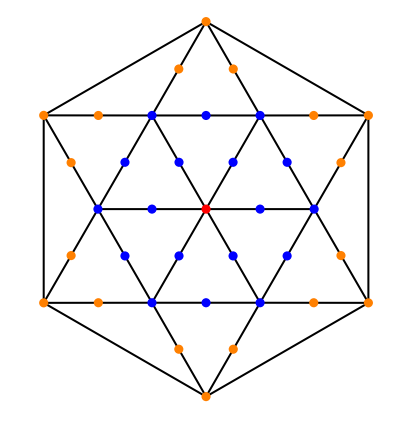
\includegraphics[width=0.2\textwidth]{figure/test.png}
	\caption{图片测试 \label{fig:scatter}}
\end{figure}

在1970年在法国尼斯举行的第十六届国际数学家大会上,罗塔提出著名的罗塔猜测(Rota's Conjecture)。该命题可简述为:对于每个有限域,都有一组有限的障碍物防止此类实现。罗塔猜测也称有限禁阵猜测;四十多年来,它在离散数学领域得到相当的关注和研究。罗塔猜测与数学领域内的拟阵论(几何的一种现代模式)具有相关性。拟阵论探究的是与我们所在世界完全不同的几何结构;该结构在投射下不会改变,而不是注重于距离和角度。例如,三个点是不是总能在一条直线上,四个点是不是总在一个平面上。罗塔猜测是一种运用数学去认识这些替代结构的方法。

\begin{table}[h!]
	\begin{center}
		\caption{一个表格}
		\begin{tabular}{ccc}
			$\alpha$ & $\beta$ & $\gamma$ \\
			\hline
			1        & 1110.1  & a        \\
		\end{tabular}
	\end{center}
\end{table}

一个由新西兰维多利亚大学数学家杰夫·惠特尔、加拿大滑铁卢大学数学家吉姆·吉伦和荷兰马斯特里赫特大学数学家伯特·杰拉德斯组成的研究团队日前宣称:他们经过15年的艰辛努力,终于找到了所有的必要的证据去证明著名的罗塔猜测。此消息一出,震惊数学界。

虽然惠特尔等人花了很长的一段时间致力于证实罗塔猜测,但另一项艰辛的工作现在才真正开始,因为他们要准备开始写工作成果。他们预计,这将需要至少三年时间才能完成写作任务。只有这样,才能让其他数学家进行验证。

对于他们的罗塔猜测证明,中国数学家和语言学家周海中认为:如果证明被确认,这将会是一个很了不起的成就;他们所使用的方法和思想也将会成为以后解决图论、拟阵论、组合论和最优化等问题的有力工具。

\bibliographystyle{abbrv}
\bibliography{./reference}

\end{document}